\typeout{------------------------------------------------------------------}
\typeout{} 
\typeout{        Fichier de base modifie par : Matth: 20 nov 2012} 
\typeout{                   sous licence GNU-GPL} 
\typeout{}
\typeout{------------------------------------------------------------------}

% Classe g�n�rale du document
   \documentclass[12pt]{report} % .10pt, 11pt, 12pt : taille de la police principale (10 par d�faut)
                 % .a4paper, letterpaper,... : d�limite la taille du papier. (letterpaper par d�faut)
	         % .fleqn : aligne les formules math�matiques � gauche au lieu de les centrer.
		 % .leqno : place la num�rotation des formules � gauche plut�t qu'� droite.
		 % .twocolumn : demande � LATEX de formater le texte sur deux colonnes.
		 % .twoside, oneside indique si la sortie se fera en recto-verso ou en recto simple.
		 % .landscape, mais il faut mettre en commentaire (ou modifier) toutes les dimmensions

% Importation de packages divers
%   \NeedsTeXFormat{LaTeX2e} 
   \usepackage[T1]{fontenc}
   \usepackage[utf8]{inputenc}		% utilisation des caract�res 8 bits en Unix (codage ISO 8859-1)
  %\usepackage[latin1]{inputenc}	% utilisation des caract�res pour Linux2
   \usepackage[usenames]{color}
   \usepackage{fancyhdr}
   \usepackage{lastpage}                % pour l'affichage du n� de la derni�re page.
   \usepackage{lmodern}
   \usepackage{multirow}                % pour l'utilisation de figures ``noy�es'' dans le texte
   \usepackage{xspace}			% package pour babel
   \usepackage[english]{babel}         % Utilisation du fran�ais (nom des sections, c�sure, ponctuation,...)
   \usepackage{amsmath,amsthm,amssymb}  % Utilisation de certains packages de AMS (cf. belles �quations)
   \usepackage{endnotes}                % Pour l'utilisation des notes en fin de documents
   \usepackage{verbatim}                % Pour l'insertion de fichier en mode verbatim
   \usepackage{portland}		% pour l'utilisation de \portrait et de \landscape sur une page
   \usepackage[pdftex]{graphicx}        % [pdftex] si utilisation d'images jgp,...
                                        % [dvips]  si utilisation d'images bmp,...
   \usepackage{pdfpages}		% Inclure des pages de pdf
   \usepackage{setspace}		% Pour d�finir un interligne
   \usepackage[bottom]{footmisc}        % Footnote at the bottom
%   \usepackage[cyr]{aeguill}		% Pour les guillemets � la Fran�aise
   \usepackage{eurosym}			% Pour les Euro
\usepackage{url}
\urlstyle{sf}
\usepackage{listings}
	
   \renewcommand{\contentsname}{Content} % si tableofcontents au d�but
   \newcommand{\Numero}{\No}
   \newcommand{\numero}{\no}
%   \newcommand{\fup}[1]{\up{#1}}

   \DeclareGraphicsExtensions{.jpg,.pdf,.mps,.png}       % d�claration d'extensions  pour les images
   %\input xy                            % pour le package xy (construction de diagramme)
   %\xyoption{all}

% Dimensions de la page :       	

  %%%%%%%%%%%%%%%%%%%%%%%%%%%%%%%%%%%%%%%%  0
  %   |                                  %
  %---+----------------------------------%  1
  %   | +----------------------------+   %  2
  %   | |          en-t�te           |   %
  %   | +----------------------------+   %  3
  %   | +----------------------------+   %  4
  %   | |                            |   %       Remarques : 
  %   | |                            |   %        . distance de '0' � '1' : un pouce + \voffset
  %   | |                            |   %        . distance de 'a' � 'b' : un pouce + \hoffset
  %   | |           texte            |   %
  %   | |                            |   %
  %   | |                            |   %
  %   | |                            |   %
  %   | +----------------------------+   %  5
  %   | +----------------------------+   %
  %   | |         bas de page        |   %
  %   | +----------------------------+   %  6
  %%%%%%%%%%%%%%%%%%%%%%%%%%%%%%%%%%%%%%%%
  %a  b c                            d  e

%    % g�n�ral
%      \voffset       0mm    % pour descendre (si positif) ou remonter (si n�gatif) le tout
%      \hoffset       0mm    % pour agrandir (si positif) ou diminuer (si n�gatif) la marge gauche (distance 'a' 'b')
      \oddsidemargin 2.5mm   % 5pt  % distance de 'b' � 'c'
%     \evensidemargin 25mm  % 15pt % distance de 'd' � 'e'
%    % texte
%      \headsep       25pt   % distance de '3' � '4', la distance entre l'en-t�te et le texte
      \textheight    220mm  % distance de '4' � '5', pour d�terminer la hauteur du texte
      \textwidth     165mm  % distance de 'c' � 'd' 
%    % en-t�te
      \topmargin     0pt    % distance de '1' � '2', pour descendre (si positif) ou remonter (si n�gatif) le tout
      \headheight    15pt   % distance de '2' � '3', doit �tre > 14.49999
%    % bas de page
      \footskip      15mm   % 30pt % distance de '5' � '6', la distance entre le texte et le bas de page
     % space for the footnode
     \setlength{\skip\footins}{1cm}
     
% Mise en page
   \pagestyle{fancy}
%   \usepackage[Matth]{fncychap}

% (Re)d�finitions diverses

  % red�finition de l'affichage des titres de section dans l'en-t�te ou le bas de page
    % remarques :
    %  .affichage du num�ro (2)    : \thesection 
    %  .affichage du nom (Section) : \sectionname
    \renewcommand{\sectionmark}[1]{\markright{\thesection.\ #1}}   % 2.2. nom de la section 2.2
    \renewcommand{\thesection}{\arabic{section}}		% II nom de la section 0.2


  % des couleurs...                   (utilisation avec par ex. \textcolor{webdarkblue}{...})
   \definecolor{codeBlue}{rgb}{0,0,1}
   \definecolor{webred}{rgb}{0.5,0,0}
   \definecolor{codeGreen}{rgb}{0,0.5,0}
   \definecolor{codeGrey}{rgb}{0.6,0.6,0.6}
   \definecolor{webdarkblue}{rgb}{0,0,0.4}
   \definecolor{webgreen}{rgb}{0,0.3,0}
   \definecolor{webblue}{rgb}{0,0,0.8}
   \definecolor{orange}{rgb}{0.7,0.1,0.1}

  % utilisation de caption, label,... pour autre chose qu'une figure
        %%%% debut macro %%%%
   \makeatletter
   \def\captionof#1#2{{\def\@captype{#1}#2}}
   \makeatother
        %%%% fin macro %%%%


% remarques : 
%  . pour mettre la date                  : \today
%  . pour mettre le nom de la section     : \rightmark
%  . pour mettre le num�ro de page        : \thepage
%  . pour mettre le nombre de pages total : \pageref{LastPage}  (mais l'�crit en rouge vu que c'est une r�f.)
%  . insertion d'une image                : \setlength{\unitlength}{1mm}
%                                             \begin{picture}(0,0)
%                                                \put(5,0){\includegraphics[scale=x.x]{xxx.xxx}}
%                                             \end{picture}

% Pour les guillemets �  la Fran�aise
\newcommand{\fermerguillemets}{\unskip\kern.15em\symbol{20}}
\newcommand{\ouvrerguillemets}{\symbol{19}\ignorespaces\kern.15em}
\let �=\fermerguillemets
\let� =\ouvrerguillemets

% Pour changer l'icone des puces : � placer juste avant une liste
 %   \renewcommand\labelitemi{\textbullet}	% Style boulet :)
 


\usepackage[pdftitle={Assignement 2},  % apparition ds les propriétés du doc
            pdfsubject={Measures and maintenance},
	    colorlinks=false,
	    linkcolor=webdarkblue, 
	    filecolor=webblue, 
	    urlcolor=webdarkblue,
	    citecolor=webgreen]{hyperref}     % pour l'utilisation des liens http,...

% Police
   \renewcommand\familydefault{ptm}        % famille normale: Times ptm
   %\renewcommand\rmdefault{phv}            % famille à utiliser pour du Roman (phv)
   %\renewcommand\sfdefault{phv}            % famille à utiliser pour du Sans Serif

% L'interligne
   % \onehalfspacing % un et demi (= \setstrech{1.5} ou = \renewcommand{\baselinestretch}{1.5})
   \renewcommand{\baselinestretch}{1.5}

% En-tete
    \lhead{\texttt{LINGI2252} - Assignement 2 - Measures and maintenance}        \chead{}        \rhead{Baufays - Colmonts (Group 6)}
    %\renewcommand{\headrulewidth}{0.5pt}     % pour l'épaisseur de la ligne

% Bas de page
    \renewcommand{\footrulewidth}{0.5pt}       % pour l'épaisseur de la ligne
    \lfoot{Partie \rightmark}        \cfoot{}        \rfoot{Page \thepage~of~7}

% TOC jusqu'au subsection
\setcounter{tocdepth}{2} % Dans la table des matieres
\setcounter{secnumdepth}{2} % Avec un numero.

\usepackage{todonotes}
\begin{document}
\begin{titlepage}
 
\begin{center}
 
% Upper part of the page
\vspace*{-2cm}
\includegraphics[width=0.10\textwidth]{ucl.png}\\[1cm]
 
\textsc{\LARGE Ecole Polytechnique de Louvain}\\[1.5cm]
 
\textsc{\Large \texttt{LINGI2252} - Software Engineering : Measures and Maintenance }\\[0.5cm]
 
 
% Title
\vspace{1.0cm}
{ \huge \bfseries Assignement 2\vspace{0.8cm}\\}
 
\vspace{1.0cm}
 
% Author and supervisor
\begin{minipage}{0.4\textwidth}
\begin{flushleft} \large
\emph{Professor :}\\
	KIM \textsc{Mens}\\
\vspace{1cm}
\emph{Program :}\\
	SINF21MS
\end{flushleft}
\end{minipage}
\begin{minipage}{0.4\textwidth}
\begin{flushright} \large
\emph{Students : (Group 6)} \\
\begin{tabular}{rl}
	Benoît \textsc{Baufays}		& {\footnotesize 22200900}\\
	Julien \textsc{Colmonts}	& {\footnotesize 41630800}\\

\end{tabular}
\end{flushright}
\end{minipage}
 
\vfill
 
% Bottom of the page
\vspace{1.1cm}
{\large Academic Year 2013-2014}
\vspace{-1cm} 
\end{center}
 
\end{titlepage}


\section{Introduction}
For the first assignment, we had to analyse the code quality of the Petit-Parser framework project. Since we had to perform this analysis manually and Petit-Parser is a quite large framework, it was a hard job to go through all the code and analysis wasn't perfect because there were too many lines of code to read through. \\
In this report, we will use some Moose tools to perform an automated code analysis of the same system. Our conclusion in the first report were optimistic about Petit-Parser even if we found some bad smells. Let's see if our previous conclusions are still valid after a deeper analysis with some metrics.

\section{Overview}
\subsection{The Moose Pyramid}
The first tool given by Moose that is visualizing feature which gives a pyramid containing general metrics of the overall system. 
\begin{figure}[ht]
\label{pyramid}
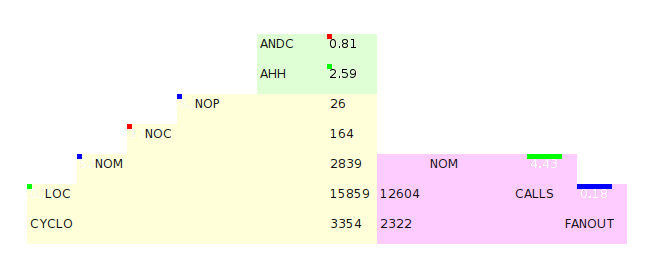
\includegraphics[scale=0.8]{overview.png}
\caption{Overview Pyramid}
\end{figure}
In this pyramid, you can observe three main blocks: one on the top and two at each side of the bottom. \\
The block on the top, in green, gives metrics about inheritance measurements. The first metric is the average number of derived classes. The little red square at the corner of this metric cell tells us that the computed number given is higher than what is known as a normal value. This could be explained. Since \textsc{PetitParser} is a framework for parsing several languages, his model is quite complex and need a large number of derived class dedicated to each kind of parsing strategy. The second metric is the average hierarchy height. Moose tells use that the value computed is close to average. Mixing the results of these two values, we can conclude that \textsc{PetitParser} uses a large number of classes which are derived in a number of levels which are still reasonable.\\
The block at the bottom left side gives several metrics about the size. The first metric shown is the number of packages. The number computed is lower than what would be expected for such a framework. But, as we already navigate manually through the code, we can say that strict rules are respected to build packages. These packages sometimes contain a large number of classes, especially the ones with tests and with parser types. The number of packages metric can be a bit distorted for this kind of framework. The second metric represents the number of classes. This time, the number is too high. To understand why this result could be a bad smell, we went back to the system browser. We saw that packages are mostly divided in two categories. There are packages that are almost empty. A very short number of classes are implemented. There are also packages with a way too many classes. After searching why these packages are too big, we found that the classes they put in them were still logically managed.  For instance, \textit{PetitParser-Parsers} package contains a large number of classes but these classes must be in this package. They are describing the different parsing strategies for the different types of parsers. The next metric is the number of methods. The number is a bit lower than what is expected. This observation comes from the fact that we have a large number of derived class. Some methods are written in a class higher in the hierarchy and don't need to be defined in all subclasses anymore. The last metric we'll take a look at is the number of lines of code. \textsc{PetitParser} seems to have this number in the average for Smalltalk projects.

\subsection{System complexity}
Before going deeper in the code, it is very interesting to identify which classes are worst than others.  To visualize this, we give, below, the System Complexity of \textsc{PetitParser}.
The height of the arrow symbolize the number of methods and the width symbolize the number of variables.
\begin{figure}[ht]
\label{system_complexity}
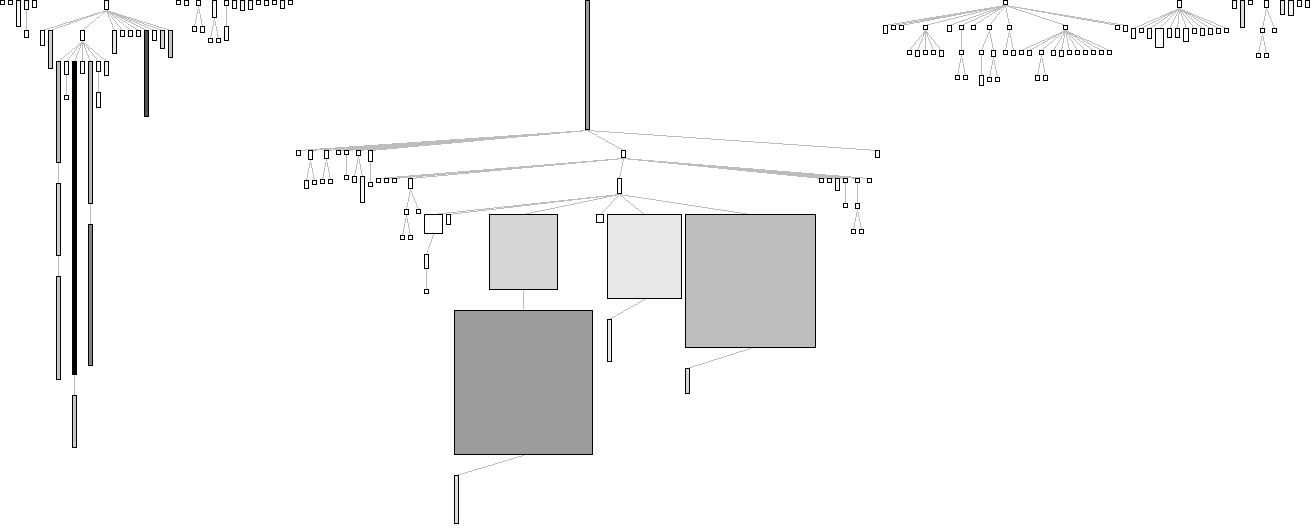
\includegraphics[scale=0.35]{system_complexity.png}
\caption{System Complexity}
\end{figure}
From left to right, we show : PPAbstractParserTest,PPParser, PJASTNode, SQLASTNode and Petit Analyzer code.  Other smalls arrows are objects from PetitParser or from SmallTalk.
We see that PPAbstractParserTest and PPParser are worst than other.  In fact, when we browse the code of this two classes, we understand the schema : for the test part, the creator of PetitParser add all his tests methods in one class.  In other hand, for the PPParser classes, and particulary for PPJavaSyntax and PetitSQLiteGrammar, he put all the variables in the same class.  When we now the syntax for Java and SQlite, we understand that the number of variables must be very important.
This graph also shows that the core of the PetitParser system is well efficient regarding to the complexity of this system.

\subsection{Blueprints Complexity}
An other tool to analyze \textsc{PetitParser} is Blueprint.  With this tool, we can show invocation of methods, access of attributes and how methods and attributes interact.\\
As we have seen before with the System complexity, the tests classes are not very efficient and we prefer to focalize on the Core of \textsc{PetitParser}.  So, you can find below a schema representing the Blueprint Complexity of \textsc{PetitParser} classes and its ecosystem.\\
\begin{figure}[ht]
\label{blueprint_system}
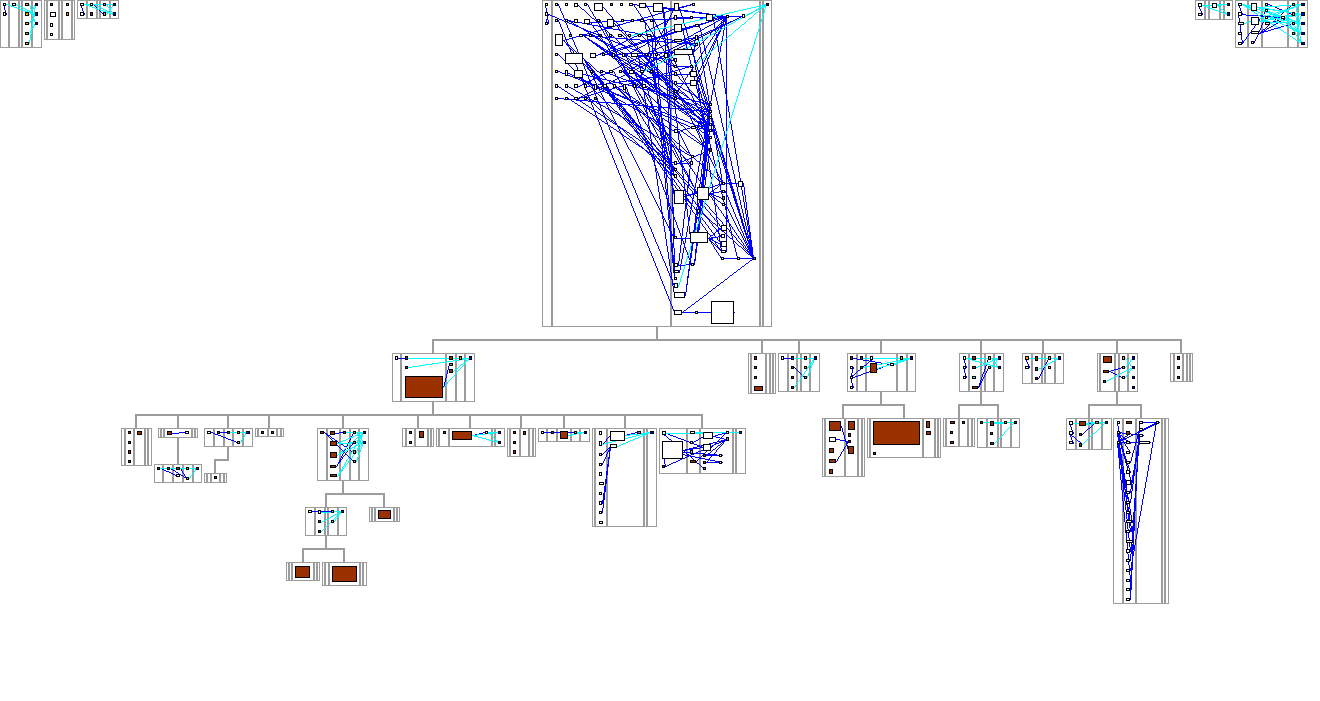
\includegraphics[scale=0.35]{blueprint_petit_parser.png}
\caption{Blueprint Complexity of PetitParser packages}
\end{figure}
This schema contains arrows representing classes and his hierarchy.  In each arrow, we found 5 columns corresponding of differents entities we found in a class.  So from left to right, we found initialization, public methods, private methods, accessors and attributes.  In each column, we have also arrows representing the entity of this type in the class.  We found also, crossing columns, dark and light blue links.  The dark link represent the invocation of methods and the light represent access to attributes.\\

In this schema, at first glance, we see that the arrow, and his tree, in the middle is the main class of \textsc{PetitParser}.  The class call \textsc{PetitParser} and, indeed, it is the main class of the project. \\

\subsubsection{Blueprints Complexity of PetitParser}
\begin{figure}[ht]
\centering
\label{blueprint_pparser}
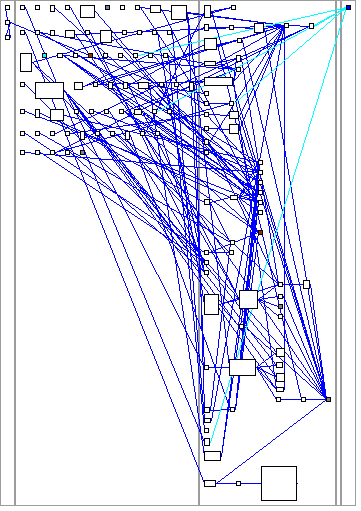
\includegraphics[scale=0.35]{blueprint_pparser.png}
\caption{Blueprint Complexity of PetitParser class}
\end{figure}
In the schema we can see more clearly the arrow representing \textsc{PetitParser} class.\\
Based on the legend explained above, we found that it contains no accessors and one attribute, \textsc{properties} which is a instanceVariable.  Some methods, public or private access directly to this attribute.  In theorical view, it's not good to access directly, you must prefer to use accessor.  With accessor, you can validate the information before setting your attributes.  Of course, it is less important for private method if you are very carefull when you use an attribute.  But, for public method, you must use a attribute.
Of course, it's a theorical view and we look all methods accessing directly the attribute before getting more analysis.  We have found 5 methods : 
\begin{itemize}
	\item removeProperty: aKey ifAbsent: aBlock : this private method 	remove the property with aKey.  If a key is found, it returns the associated value and the the result of evaluating aBlock otherwise.  According to the code, we can say that this method is a safe method for the attribute : it removes the key if, and only if, the key exists.  With this solution, the integrity of the attribute is checked;
	\item propertyAt: aKey put: anObject : this private method change the object (anObject) linked to the key (aKey) in the property.  if aKey is not found, it creates a new entry.  Again, we see that this method is a safe method and the integrity of the attribute is checked;
	\item propertyAt: aKey ifAbsent: aBlock : this private method give the value associated to aKey if aKey is a key in property and answer the result of evaluating aBlock otherwise.  Like the first method, we see that the integrity of the attribute is checked ;
	\item postCopy : this public method give a copy of the property.  To perform this copy, it is normal to access to the attribute but, for a public method, it's preferable to use a getter, event if we don't change it ;
	\item hasProperty: aKey : this public method test if aKey is a key in the property.  Also, like the previous public method, the integrity of the attribute is checked but it's not good to access directly to an attribute in a public method.
\end{itemize}
In ddition to checking the code of methods, it is interesting to note that this methods are well used by this class or children classes.\\
Even if the integrity of the attribute is checked in every method accessing directly to the attribute, we see that almost method performs a test on property.  Why the creator doesn't use the test method in other methods listed below ? \\
Finally, we see that some methods are setter for property.  Because property contains keys and values, the creator can not do a "simple" setter to change the property but he create method to add or remove (key,value).  So, in conclusion, we can see that it's important to check the code after reading this schema and, evenf if we found no getter and setter, the most methods accessing directly the attribute are setter and getter for the structure of property.\\

For the dark blue links, we see that a lot of methods are linked together.  It's a signe that the code are modulable and reduce code duplication.  It is also the consequence of the \textsc{PetitParser} system : it uses structures with childrens and list of object.  To access these structures,  methods use these sub-structures and methods related to them.\\

Finally, we see some brown arrows.  It means that the method override code.  AND ???? \\

\subsection{Duplication side-by-side}
Moi, Moose me renvoit un schéma vide, WTF ?

\subsection{Bad smells}
With the Moose tool, we can have metrics about almost everything but they are not all relevant to detect bad smells.  To Detect more precisly some bad smells, we have created some query to get bad methods.\\

\subsubsection{Number of lines of Code}
First, we want to see methods where the number of lines of codes is bigger than 50, we can query :
\begin{lstlisting}
each numberOfLinesOfCode>50
\end{lstlisting}
With this query, we can see that, in the \textsc{PetitParser} System, we found 7 classes with more than 50 lines of codes.\\

\begin{figure}[ht]
\centering
\label{system_complexity_big_classes}
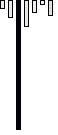
\includegraphics[scale=0.55]{system_complexity_big_methods.png}
\caption{Complexity of big classes}
\end{figure}
In the schema below, we can see that the class PPParser is the bigger one, with 758 lines of codes.  To go depper in the analysis, we can perform the query for this class and we see \todo{plante chez moi}\\
\subsubsection{Accessors}
An other interresting metric is the number of getter and setter for one attribute.  In mai ncase, you must have one getter and one setter for every attribute.  We see before that, for some attributes, we don't have any accessors. \\
\begin{lstlisting}
each numberOfAccessorMethods >= ( 2 * each numberOfAttributes ) 
\end{lstlisting}
This query return 22 classes and we can visualize these with the blueprint schema.\\
\begin{figure}[ht]
\centering
\label{more_access_blueprint}
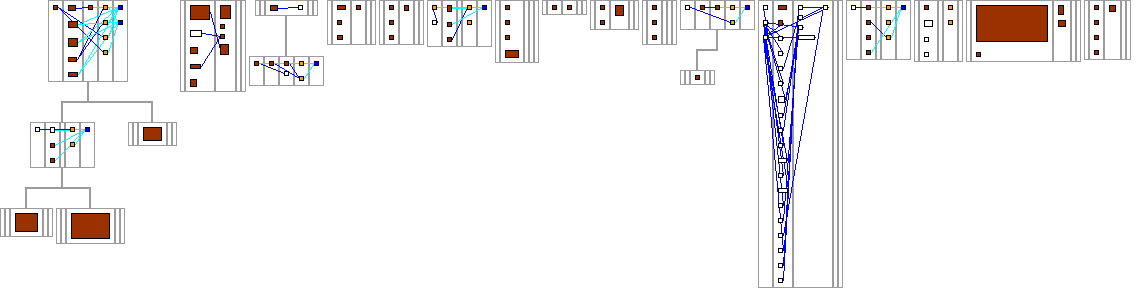
\includegraphics[scale=0.35]{more_access_blueprint.png}
\caption{Blueprint of classes with more accessors than 2* attributes}
\end{figure}


\todo{duplication side-by-side}
\todo{CityMap}


\end{document}

